\section{Results}
\label{sec:results}
The gate passes, all 90 fits converged, and all three pre-registered contrasts resolve in the predicted direction. This section reports the gate first, then the damages of the derived orders, and then the per-class recall changes behind them.

\subsection{The repaired score passes the gate}
\label{sec:gate-results}
G1 and G2 both hold. The hard-tail order scores 350, the easy-tail order 453, and the 30 random orders 604 on average, with a range of 475 to 772; the order of the three scores matches the observed damages, 1.59, 2.41 and 2.91 points. G3 is positive: across the random orders, score and single-fit damage correlate at a Spearman coefficient of 0.58 ($p<0.001$, $n=30$), and at 0.52 when each order is predicted from a line fitted without it. This is at the ceiling of about 0.57 that single-fit noise allows (Section~\ref{sec:gate}).

The calibration line fitted to the random orders, $D = -0.01 + 0.00485\,S$, predicts 2.18 points for the easy-tail order and 1.68 points for the hard-tail order. Both lie inside the observed intervals, 1.95 to 2.85 and 1.22 to 1.95 points. For the three derived orders it predicts 4.34 points (worst), 3.68 points (flip) and 0.97 points (mild). The worst and mild orders score 898 and 203, which lie 4.0 and 5.5 standard deviations of the random-order scores above and below their mean, so both predictions extrapolate well beyond the range on which the line was fitted.

\subsection{Derived orders span 1.3 to 4.5 points of damage}
\label{sec:damage}
Table~\ref{tab:damage} lists the damage of every fixed order together with the random-order average. The worst order costs 4.51 points, more than any other fixed order and more than all but one of the 30 single random fits, whose damages range from 1.53 to 4.69 points. The mild order costs 1.34 points, the lowest of the fixed orders, and close to the 1.18 points of the native-distribution arm of the prevalence curve. The ranking worst $>$ flip $>$ random $>$ easy $>$ hard $>$ mild holds in each of the three splits separately.

\begin{table}[htbp]
\centering
\small
\setlength{\tabcolsep}{6pt}
\renewcommand{\arraystretch}{1.08}
\begin{tabular}{@{}lrrrl@{}}
\toprule
Class order & $S$ & Predicted $D$ & Observed $D$ (pp) & Source \\
\midrule
Worst (argmax $S$) & 898 & 4.34 & 4.51 \; (3.93 to 5.08) & this report \\
Flip (reversed worst) & 761 & 3.68 & 3.41 \; (2.98 to 3.84) & this report \\
Random, mean over 30 orders & 604 & 2.91 & 2.91 \; (2.48 to 3.34) & prevalence curve \\
Easy-tail & 453 & 2.18 & 2.41 \; (1.95 to 2.85) & tail assignment \\
Hard-tail & 350 & 1.68 & 1.59 \; (1.22 to 1.95) & tail assignment \\
Mild (argmin $S$) & 203 & 0.97 & 1.34 \; (1.00 to 1.69) & this report \\
\bottomrule
\end{tabular}
\caption{The score orders all six assignments by damage, and a line fitted only on random orders predicts every fixed order within 0.37 points. $S$ is Equation~\eqref{eq:score} at $\rho=100$. Predicted $D$ comes from the calibration line fitted to the 30 random orders before the derived orders were fitted; the random-order row is fitted, not predicted. Observed $D$ is the loss of test patient-macro balanced accuracy against r1, pooled over 30 fits, with 95 percent bootstrap intervals. Random and sorted orders are reused from \citet{queisler2026prevalenceTcga} and \citet{queisler2026tailTcga}.}
\label{tab:damage}
\end{table}

\noindent Table~\ref{tab:contrasts} gives the pre-registered contrasts. \textbf{H1} holds: the worst order costs 1.60 points more than a random order, with an interval of 1.11 to 2.08 points that lies entirely above the one-point threshold. \textbf{H2} holds: the mild order costs 1.57 points less than a random order, with an interval of 1.11 to 2.03 points, likewise above the threshold. The two effects are nearly symmetric around the random average, and the full range between the worst and the mild order is 3.17 points, larger than the 2.91 points the ratio costs on average.

\textbf{H3} holds as well: the worst order costs 1.11 points more than its reversal, with an interval of 0.47 to 1.73 points. This contrast was expected to be the hardest to resolve, since the line predicted only 0.66 points. The flip order separates each confused pair by exactly the same number of ranks as the worst order, so the difference is due to which member of each pair receives the larger allocation. At the same time, the flip order lies 0.49 points above the random average, a difference without a pre-registered interval but consistent with separation alone, regardless of direction, carrying part of the effect.

The descriptive comparison of the mild and hard-tail orders stays unresolved, at $-0.25$ points ($-0.58$ to $0.09$), as expected from a predicted difference of $-0.71$ points and a paired interval half-width of about 0.35 points.

\begin{table}[htbp]
\centering
\small
\setlength{\tabcolsep}{6pt}
\renewcommand{\arraystretch}{1.08}
\begin{tabular}{@{}llrl@{}}
\toprule
Endpoint & Contrast & Estimate (pp) & 95\% interval \\
\midrule
H1 & $D_{\text{worst}} - D_{\text{r100}}$ & 1.60 & 1.11 to 2.08 \\
H2 & $D_{\text{r100}} - D_{\text{mild}}$ & 1.57 & 1.11 to 2.03 \\
H3 & $D_{\text{worst}} - D_{\text{flip}}$ & 1.11 & 0.47 to 1.73 \\
Descriptive & $D_{\text{mild}} - D_{\text{hard}}$ & $-0.25$ & $-0.58$ to $0.09$ \\
\bottomrule
\end{tabular}
\caption{All three pre-registered contrasts exclude zero, and H1 and H2 exceed the one-point threshold with their whole interval. Paired contrasts of balanced-accuracy damage at $\rho=100$, pooled over 30 fits per arm with 95 percent bootstrap intervals.}
\label{tab:contrasts}
\end{table}

\noindent Figure~\ref{fig:score} places the fitted orders against the random cloud. The derived orders lie on the extension of the random-order trend at both ends. Regressing the observed on the predicted damage of the five fixed orders gives a slope of 0.92, and the mean absolute prediction error is 0.23 points over all five and 0.27 points over the three derived orders alone. The line does not overshoot at the upper extreme, as the extrapolation caveat anticipated; it underestimates the worst order by 0.17 points and overestimates the flip order by 0.27 points. Its largest miss is the mild order, observed at 1.34 points against a prediction of 0.97, just below the lower end of the interval at 1.00. Damage therefore flattens at the mild end: minimizing the score further does not keep lowering the damage at the rate the line implies.

\begin{figure}[htbp]
\centering
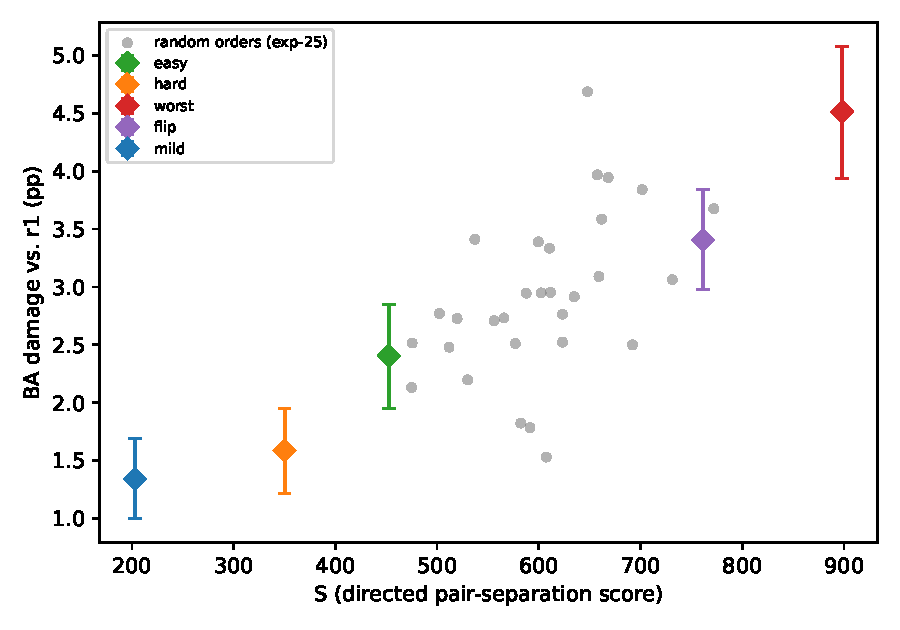
\includegraphics[width=0.78\textwidth]{damage_vs_score_r100.pdf}
\caption{The derived orders extend the random-order trend in both directions. Observed balanced-accuracy damage against the rate-weighted score at $\rho=100$. Grey points: the 30 random class orders of the prevalence curve, one per fit. Diamonds with 95 percent bootstrap intervals, each pooled over 30 fits: hard-tail (orange) and easy-tail (green) orders of the tail-assignment study, and the mild (blue), flip (purple) and worst (red) orders fitted here.}
\label{fig:score}
\end{figure}

\subsection{Recall moves with allocation relative to the confusion partner}
\label{sec:recall}
The damage of the worst order is concentrated. Nine classes lose more than ten points of recall under it, against two under the mild order, and the largest single loss is 42.8 points against 13.2 points. Table~\ref{tab:pairs} follows the main confused pairs through the three derived orders.

\begin{table}[htbp]
\centering
\small
\setlength{\tabcolsep}{5pt}
\renewcommand{\arraystretch}{1.08}
\begin{tabular}{@{}llrrrrrr@{}}
\toprule
& & \multicolumn{2}{c}{Worst} & \multicolumn{2}{c}{Flip} & \multicolumn{2}{c}{Mild} \\
\cmidrule(lr){3-4}\cmidrule(lr){5-6}\cmidrule(l){7-8}
Class & $h_c$ (\%) & Rank & $\Delta$ & Rank & $\Delta$ & Rank & $\Delta$ \\
\midrule
COAD & 51.5 & 2 & $+27.8$ & 27 & $-34.1$ & 28 & $-11.0$ \\
READ & 60.6 & 27 & $-42.8$ & 2 & $+22.0$ & 29 & $-4.0$ \\
\addlinespace
LUSC & 54.5 & 0 & $+21.4$ & 29 & $-37.8$ & 23 & $-9.2$ \\
HNSC & 69.0 & 19 & $-15.1$ & 10 & $+1.6$ & 24 & $-5.9$ \\
CESC & 46.7 & 29 & $-27.2$ & 0 & $+17.3$ & 22 & $-0.9$ \\
LUAD & 65.3 & 26 & $-19.2$ & 3 & $+11.0$ & 16 & $+2.5$ \\
\addlinespace
LGG & 78.8 & 5 & $+8.7$ & 24 & $-12.7$ & 8 & $+1.0$ \\
GBM & 77.0 & 24 & $-16.4$ & 5 & $+9.1$ & 9 & $+1.5$ \\
\addlinespace
LIHC & 85.5 & 8 & $+1.5$ & 21 & $-7.0$ & 5 & $+1.8$ \\
ACC & 72.9 & 28 & $-26.3$ & 1 & $+7.0$ & 6 & $+3.4$ \\
\bottomrule
\end{tabular}
\caption{Classes placed far below their main confusion partner lose large amounts of recall, and the loss is not symmetric within a pair. $h_c$ is balanced-arm recall; rank 0 holds 2,843 patches and rank 29 holds 28; $\Delta$ is the pooled change in own recall against r1, in points. Groups are confused pairs or clusters: colon and rectum adenocarcinoma; lung squamous cell, head and neck squamous cell, cervical squamous cell carcinoma and lung adenocarcinoma, all confused with lung squamous cell carcinoma; lower-grade glioma and glioblastoma; liver hepatocellular and adrenocortical carcinoma.}
\label{tab:pairs}
\end{table}

\noindent Within every group, the member placed far below its partner loses recall and the member placed above it gains, and the roles exchange when the order is reversed. Rectum adenocarcinoma loses 42.8 points at rank 27 below colon adenocarcinoma and gains 22.0 points at rank 2 above it. In the mild order both sit in the tail, at ranks 28 and 29, and lose 11.0 and 4.0 points, far less than either loses when separated from the other. The squamous cluster and the gliomas behave in the same way.

The direction effect of H3 is visible in the asymmetry within pairs. Adrenocortical carcinoma loses 26.3 points when it sits at rank 28 below hepatocellular carcinoma, whereas hepatocellular carcinoma loses only 7.0 points in the reversed position. The two classes are each other's main confusion partner, but under balanced training adrenocortical carcinoma is misclassified far more often, with a recall of 72.9 against 85.5 percent; the rate-weighted score encodes this asymmetry through $w_{c\rightarrow d}$. Figure~\ref{fig:pairs} generalizes the table to all 30 classes: under the mild order almost every class sits within a few ranks of its main confusion partner and its recall change stays within 13 points, whereas under the worst order half of the classes sit 15 or more ranks from their partner and recall changes spread from $-43$ to $+28$ points.

\begin{figure}[htbp]
\centering
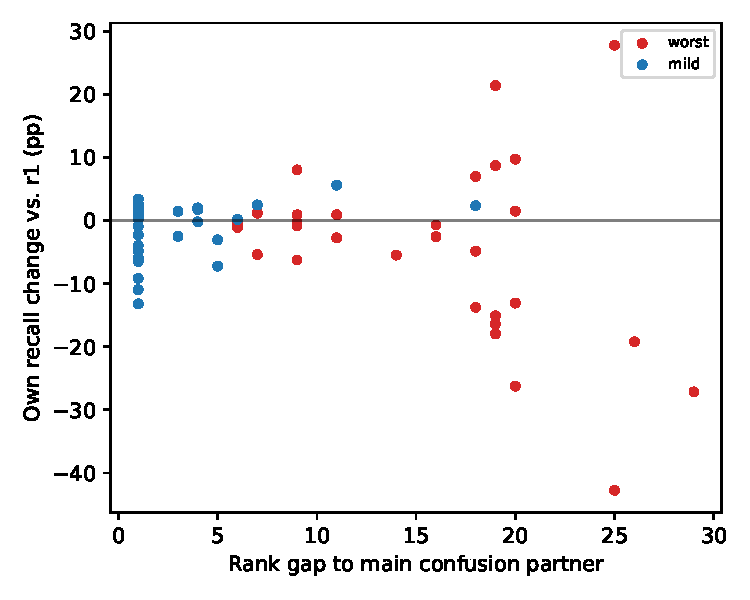
\includegraphics[width=0.62\textwidth]{pair_gap_r100.pdf}
\caption{Recall changes spread widely only when a class is far in rank from its main confusion partner. Each point is one class under the worst (red) or mild (blue) order: the rank gap to the class it is most often predicted as in the balanced arm, against the pooled change in its own recall against r1.}
\label{fig:pairs}
\end{figure}

\section{Discussion}
\label{sec:discussion}
The mechanism that the tail-assignment study read off two fitted orders \citep{queisler2026tailTcga} now predicts damage. A single scalar over class orders, fitted on random orders alone, ranks six assignments correctly and predicts the damage of three assignments it was never fitted on within 0.37 points. The orders it produces move the damage by 1.6 points in each direction around the random average, and each of these shifts exceeds the one-point threshold of the series with its whole interval. The pairwise account is therefore not only a description of which classes moved in one experiment. It is a quantitative predictor of how much a whole assignment costs.

Two parts of that account are separately supported. Separation of confused pairs matters: the flip order separates them as far as the worst order and is still more damaging than a random order. Direction matters as well: which member of a pair holds the larger allocation accounts for another 1.11 points. The per-class results explain both effects. A class that is often predicted as a well-supported partner gives up recall to it, and the size of the loss depends on how often the balanced classifier already makes that error and how much recall the class has. The class at the tail does not need to be difficult on its own; rectum adenocarcinoma and adrenocortical carcinoma lose most of their recall only when their specific partner is abundant.

The contrast with the failed score is instructive. The two scores differ only in whether a class's confusion weights sum to one or to its error rate. With row-normalized weights, a class the classifier almost never confuses still contributed a full unit of weight, and the score responded to the monotone alignment of recall and rank that sorting creates \citep{queisler2026worstTcga}. With rate weights, such a class contributes almost nothing, and the score responds to where confusion actually occurs. The worst order it produces is essentially unrelated to difficulty, with a correlation of 0.08 between rank and balanced recall.

For the questions of this series, the result reframes the damage of a long-tailed allocation. At $\rho=100$ and a fixed budget, the random-order average of 2.91 points is one point on a range of at least 1.34 to 4.51 points spanned by the assignment alone. Which classes are rare is thus as consequential as how rare they are. The practical corollary is that a long-tailed data set can be more or less harmful depending on whether confused classes are rare together or apart, and that the balanced classifier's confusion rates indicate in advance which case applies. The mild end of the range is the less certain one: the damage there flattens below the line, which suggests that some cost of the ratio cannot be removed by any assignment.

\section{Limitations}
\label{sec:limitations}
The score was chosen after exploratory checks on stored outputs, among about nine variants, and the easy-tail and hard-tail anchors informed that choice. Its agreement with those two anchors is therefore not an independent test. The three derived orders are, since they were fixed and their predictions recorded before any of them was fitted; but they are three orders, derived from the same score, and they cannot establish how well the score ranks the space of assignments between them.

The worst and mild orders are local extremes found by hill climbing, not proven optima. Some assignment may be more damaging than the worst order reported here, so 4.51 points is a lower bound on the worst case rather than an estimate of it. The score inputs, confusion rates and balanced recall, are taken from balanced-arm predictions on the same test patients on which damage is evaluated. This is appropriate for a study of mechanism, but a practitioner would have to estimate confusion from validation data, and the predictive accuracy reported here is an upper bound for that setting.

All derived orders were fitted at $\rho=100$. The score's ordering of assignments does not depend on the ratio, but whether the damage ordering carries over to milder ratios is not tested, and the single-fit noise of the random orders caps the within-family correlation that any score can reach. All results are conditional on twenty patients per class, frozen Virchow2 features, multinomial logistic regression, and the three overlapping splits of TCGA-UT; on data sets whose classes collapse in the tail, such as BRACS, headroom rather than confusion structure dominated \citep{queisler2026tailBracs}, and the score has not been tested there.
